\chapter{\IfLanguageName{dutch}{Proof-of-concept}{Proof-of-concept}}%
\label{ch:proof-of-concept}
\section{\IfLanguageName{dutch}{Virtuele omgeving}{Virtual environment}}%
\label{sec:Virtuele_omgeving}

Voor het opzetten van een oplossing en deze te kunnen testen en evalueren, is er een virtuele omgeving opgezet.
Deze virtuele omgeving is opgezet in GNS3, een netwerkemulator die het mogelijk maakt om netwerkapparatuur alsook virtuele machines te simuleren.
Binnen deze virtuele omgeving zal er aan netwerksegmentatie gedaan worden, het netwerk zal opgedeelde worden in 3 segmenten: een Admin, DMZ en employee segment.
Binnen het Admin segment zullen grotendeels van de servers staan alsook een workstation, in het DMZ segment zal er 1 server staan en in het employee segment zullen de werkstations staan.
Deze segmentatie bestaat met als doel om het aantal vertrouwde root certificaten te beperken tot de benodigdheden van de verschillende segmenten, zo worden er minder root certificaten vertrouwd door de verschillende segmenten wat tot lagere security risico's leidt.
Binnen het Admin segment staan er 4 servers, "Windowsserver", "Database", "CA" en "Vault" alsook is hier een workstation "Admin-client". Het DMZ segment heeft een server "Webserver" en het employee segment heeft 1 workstation "Employee-client". \\

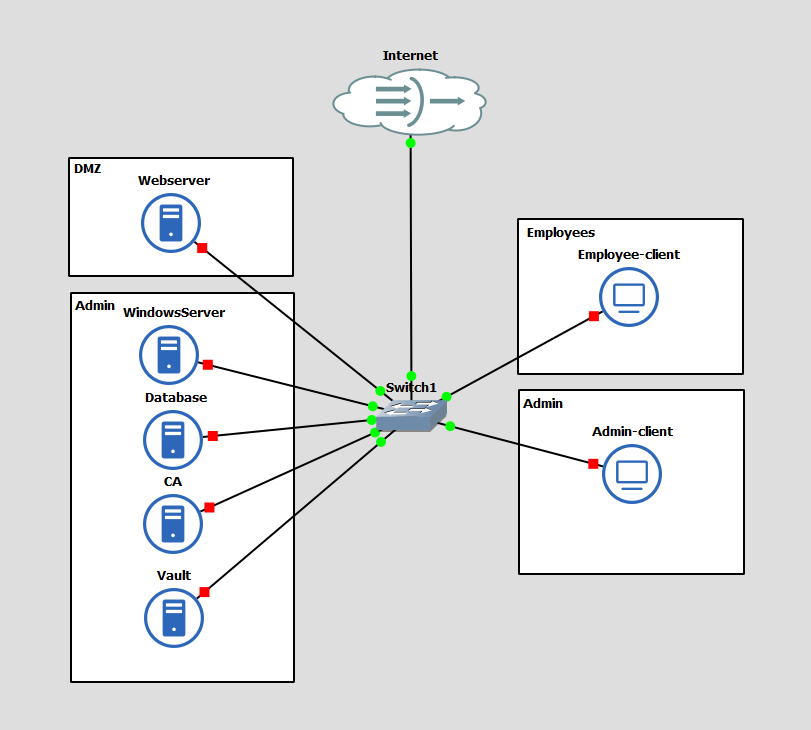
\includegraphics[width=1\textwidth]{Architectuurplan.png}

\subsection{\IfLanguageName{dutch}{Webserver}{Webserver}}
\label{subsec:Webserver}

De webserver draait op Ubuntu 22.04 en heeft een Nginx webserver draaien met een certificaat dat ondertekend werd door de CA server van binnen deze virtuele omgeving.
Het doel van deze webserver is om de functionaliteit van het aanpassen van de truststore te testen, als een end-point de webpagina kan bereiken zonder waarschuwing via het https protocol, dan betekent dat de server "CA" zijn root certificaat aanwezig is in de end-point zijn truststore.

\subsection{\IfLanguageName{dutch}{Windows server}{Windows server}}
\label{subsec:Windows_server}

Deze server draait Windows Server 2022 en is de domein controller van de virtuele omgeving. Het domein is "Bachelorproef.local" en de server heeft een Active Directory (AD) opgezet. De Active Directory bevat 2 logins voor de Windows clients "Employee1" en "Admin1". Binnen de AD zal elke Windows client die het netwerk betreedt automatisch gestoken worden. 
Deze clients worden manueel in de juiste organisational unit (OU) gestoken. In dit geval zijn dit de OU "Employee" en "Admin".

\subsection{\IfLanguageName{dutch}{CA}{CA}}
\label{subsec:CA}

De CA server draait een Almalinux 8.8 image en is een Certificate Authority (CA). Het root certificaat is gemaakt met OpenSSL en is ondertekend door de CA zelf. Zoals eerder vermeld is er een leaf certificaat aangemaakt en ondertekend voor de webserver.

\subsection{\IfLanguageName{dutch}{Vault}{Vault}}
\label{subsec:Vault}

De Vault server draait ook Ubuntu 22.04 en heeft een Hashicorp Vault server draaien. Deze vault server zal gebruikt worden om de root certificaten op een centrale plaats op te slaan.

\subsection{\IfLanguageName{dutch}{Employee-client}{Employee-client}}
\label{subsec:Employee-client}

Deze Windows client draait Windows 11, en bevindt zich in het Employee netwerksegment. Deze client maakt deel uit van het domein "Bachelorproef.local" en is ook lid van de OU "Employee".

\subsection{\IfLanguageName{dutch}{Admin-client}{Admin-client}}
\label{subsec:Admin-client}

Deze Windows client draait ook Windows 11 en bevindt zich in het Admin netwerksegment. Deze client maakt ook deel uit van het domein "Bachelorproef.local" en is ook lid van de OU "Admin".

\section{\IfLanguageName{dutch}{Eerste oplossing}{First solution}}%
\label{sec:Eerste_oplossing}
\subsection{\IfLanguageName{dutch}{Oplossing voor Windows end-points door middel van GPO's met root certificaten}{Solution for Windows end-points using GPOs with root certificates}}
\label{subsec:Oplossing_voor_Windows_end-points_door_middel_van_GPOs_met_root_certificaten}
Om Windows clients hun truststores centraal te kunnen beheren, kan er simpelweg een GPO (Group Policy Object) aangemaakt worden die root certificaten bevat en deze kan dan toegepast worden op een OU binnen de Active Directory.
Er kan dus een GPO aangemaakt worden per OU (in dit geval de 3 OU's voor de 3 netwerksegmenten) die elk de juiste root certificaten bevatten.
Voor deze proof of concept zal er een verzameling van root certificaten opgeslagen worden in een directory op de Windows server, deze directory zal 3 subdirectories bevatten voor elk netwerksegment. De root certificaten die in deze subdirectories staan zijn de root certificaten die de clients in dat netwerksegment moeten vertrouwen.
De GPO's zullen dan de root certificaten uit deze subdirectories halen en deze toevoegen aan de truststore van de clients in dat netwerksegment.
De GPO's kunnen als volgt aangemaakt worden:
\begin{itemize}
    \item Open de Group Policy Management Console (GPMC) op de Windows server.
    \item Maak een nieuwe GPO aan door met de rechtermuisknop op de OU te klikken en "Create a GPO in this domain, and Link it here" te selecteren.
    \item Geef de GPO een naam, bijvoorbeeld "Employee-certificates".
    \item Klik met de rechtermuisknop op de GPO en selecteer "Edit".
    \item Ga naar Computer Configuration > Policies > Windows Settings > Security Settings > Public Key Policies > Trusted Root Certification Authorities.
    \item Klik met de rechtermuisknop en selecteer "Import".
    \item Volg de wizard om het root certificaat te importeren vanuit de directory op de Windows server.
    \item Herhaal deze stappen voor de andere OU's en root certificaten.
\end{itemize}

De GPO's kunnen dan toegepast worden, dit kan door met de rechtermuisknop op de OU te klikken en "Link an Existing GPO" te selecteren. Selecteer dan de GPO die je wilt toepassen op de OU. \\

Op de clients kan je dan de GPO's toepassen door het volgende commando uit te voeren in de command prompt:
\begin{minted}{powershell}
    gpupdate /force
\end{minted}
Ook kan de GPO toegepast worden door de clients opnieuw op te starten. \\

\subsection{\IfLanguageName{dutch}{Oplossing voor Linux end-points met Ansible}{Solution for Linux end-points using Ansible}}
\label{subsec:Oplossing_voor_Linux_end-points_met_Ansible}
Om het probleem van het centraal beheren van de root certificaten op te lossen, kan er een Ansible playbook gemaakt worden dat root certificaten kan toevoegen aan de truststores van de Linux systemen.
De CA server zal in deze proof-of-concept ook de Ansible control server zijn. Dit is de server die de Ansible playbooks zal uitvoeren op de end-points.
Hiervoor is een inventory bestand nodig dat de IP adressen van de end-points bevat alsook de locatie van de key en gebruiker die gebruikt zal worden voor de SSH verbinding. Dit bestand voor deze omgeving ziet er als volgt uit:
\begin{minted}{yaml}
    [DMZ]
    web ansible\_host=bpweb.bachelorproef.local ansible\_user=ubuntu ansible\_ssh\_private\_key\_file=/home/almalinux/.ssh/id\_rsa

    [Admin]
    db ansible\_host=db.bachelorproef.local ansible\_user=almalinux ansible\_ssh\_private\_key\_file=/home/almalinux/.ssh/id\_rsa
    ca ansible\_host=ca.bachelorproef.local ansible\_user=almalinux ansible\_ssh\_private\_key\_file=/home/almalinux/.ssh/id\_rsa
\end{minted}

Net zoals bij de Windows server zal er een directory aangemaakt worden op de server "CA" die subdirectories bevat voor elk netwerksegment. Deze subdirectories bevatten de root certificaten die de end-points in dat netwerksegment moeten vertrouwen.
Met deze bestanden en directories kan er een Ansible playbook gemaakt worden dat de root certificaten uit de juiste subdirectory haalt en toevoegt aan de truststore van de end-points. Dit kan gedaan worden met het volgende Ansible playbook:
\begin{minted}{yaml}
    - name: Installeer en vervang alle root certificaten per groep
        hosts: all
        become: true
        vars:
        cert\_source\_dir: >-
            {{ '/home/almalinux/Ansible/DMZ' if 'DMZ' in group\_names else '/home/almalinux/Ansible/Admin' }}
        dest\_cert\_dir: >-
            {{ '/usr/local/share/ca-certificates' if ansible\_os\_family == "Debian" else '/etc/pki/ca-trust/source/anchors' }}
        update\_command: >-
            {{ 'update-ca-certificates' if ansible\_os\_family == "Debian" else 'update-ca-trust extract' }}
    
        tasks:
    
        ### BACKUP STANDAARD TRUSTSTORE ###
        - name: Maak back-up van standaard truststore op Debian
            when: ansible\_os\_family == "Debian"
            command: >
            tar czf /root/debian-ca-certificates-backup.tar.gz /usr/share/ca-certificates /etc/ssl/certs
    
        - name: Maak back-up van standaard truststore op RedHat
            when: ansible\_os\_family == "RedHat"
            command: >
            tar czf /root/redhat-ca-certificates-backup.tar.gz /etc/pki/ca-trust
    
        ### VERWIJDER STANDAARD CERTIFICATEN ###
        - name: Ledig standaart truststore op Debian
            when: ansible\_os\_family == "Debian"
            file:
            path: "{{ item }}"
            state: absent
            loop:
            - /usr/share/ca-certificates/mozilla
            - /etc/ssl/certs/ca-certificates.crt
    
        - name: Ledig standaart truststore op RedHat
            when: ansible\_os\_family == "RedHat"
            shell: rm -f /etc/pki/ca-trust/source/anchors/*
            args:
            warn: false
    
        ### CERTIFICATEN INSTALLEREN ###
        - name: Zoek alle certificaten in groepsspecifieke map
            find:
            paths: "{{ cert\_source\_dir }}"
            patterns: "*.crt"
            register: certs\_to\_install
    
        - name: Kopieer certificaten naar truststore directory
            copy:
            src: "{{ item.path }}"
            dest: "{{ dest\_cert\_dir }}/{{ item.path | basename }}"
            owner: root
            group: root
            mode: '0644'
            loop: "{{ certs\_to\_install.files }}"
            when: certs\_to\_install.matched > 0
    
        ### TRUST STORE UPDATEN ###
        - name: Update systeem truststore
            command: "{{ update\_command }}"
    
        ### VERIFICATIE ###
        - name: Bevestiging
            debug:
            msg: "Alle root certificaten zijn geïnstalleerd en de truststore is bijgewerkt!" 
\end{minted}

De playbook begint met het maken van een back-up van de standaard out-of-the-box truststores, dit is belangrijk aangezien de tweede stap deze zal leegmaken. Moest een belangrijke root certificaat ontbreken na het uitvoeren van de playbook, kan deze teruggezet worden met de back-up.
Deze playbook kijkt vervolgens naar welke groep de end-point inzit om zo de certificaten uit de directory met dezelfde naam te halen, daarna worden de certificaten gekopieerd naar de directory op de end-points die de truststores bekijken en tenslotte wordt de truststore geüpdatet met het juiste commando. 
Deze playbook bepaalt de bestemmingsdirectory en het update commando op basis van de 'OS family' van de end-point.
In dit geval is dit Debian of Red Hat, voor andere OS families zouden deze nog manueel moeten worden toegevoegd samen met de juiste commando's en directories. \\

Om het voorgaande Ansible playbook uit te voeren, kan er gebruik gemaakt worden van de volgende commando's:
\begin{minted}{bash}
    ansible-playbook -i inventory playbook.yml
\end{minted}

Waarbij "inventory" het inventory bestand is dat de IP adressen van de end-points bevat en "playbook.yml" het Ansible playbook is dat de root certificaten toevoegt aan de truststores van de end-points. \\

\subsection{\IfLanguageName{dutch}{Pro's en Con's van de eerste oplossing}{Pro's and Con's of the first solution}}
\label{subsec:Pros_en_Cons_van_de_eerste_oplossing}
\begin{itemize}
    \item Pro's:
    \begin{itemize}
        \item De root certificaten kunnen eenvoudig beheerd worden.
        \item Geen nodige installatie van extra software op de end-points.
        \item End-points ondervinden geen hinder van de installatie van de root certificaten.
        \item Er zijn weinig points of failure aangezien de oplossing geen bijkomende servers of software nodig heeft.
    \end{itemize}
    \item Con's:
    \begin{itemize}
        \item De GPO's passen alleen maar toe wanneer de end-points opnieuw opgestart worden of de GPO's geforceerd worden.
        \item Het importeren van root certificaten in de GPO's kan niet geautomatiseerd worden, dit betekent dat als er veel root certificaten zijn, het handmatig aanmaken van de GPO's tijdrovend zal zijn.
        \item De certificaten staan in directories die niet beveiligd zijn, dit brengt een risico mee dat de certificaten binnen de directory kunnen worden aangepast of verwijderd.
        \item Zowel de Windows server als de CA server (de Ansible control server) hebben een kopie van de root certificaten, bij een aanpassing van de root certificaten moeten deze op beide servers aangepast worden.
        \item De Ansible playbook is niet schaalbaar, een server maakt SSH verbindingen met de end-points en voert de playbook uit op elke end-point. Dit betekent dat als er veel end-points zijn, de Ansible playbook traag zal zijn en mogelijk niet alle end-points kan bereiken.
    \end{itemize}
\end{itemize}

\section{\IfLanguageName{dutch}{Tweede oplossing}{Second solution}}%
\label{sec:Tweede_oplossing}
\subsection{\IfLanguageName{dutch}{Installeren van een Vault server}{Installing a Vault server}}
\label{subsec:Installeren_van_een_Vault_server}

Om het probleem van het dubbel beheren van de root certificaten op te lossen, moet er een centraal punt op het netwerk zijn die de root certificaten bevat. Dit kan gedaan worden door een Hashicorp Vault server op te zetten. Deze server brengt naast het beheren van de root certificaten ook autorisatie met zich mee waardoor de certificaten ook beveiligd zijn.
Binnen deze proof-of-concept omgeving is er een standalone server voorzien voor Hashicorp Vault genaamd "Vault". Deze server heeft een kopie van de directories met root certificaten die op de server "CA" stond. Daarnaast zal Vault in "dev" mode draaien, dit is een testmodus die het mogelijk maakt om snel te experimenteren met Vault zonder dat er een volledige configuratie nodig is. 
In deze modus zal de vault server ook geen persistentie hebben, wat betekent dat alle gegevens uit de vault verloren gaan als de vault sluit of de server stopt.

De vault server wordt opgestart met de volgende commando:
\begin{minted}{bash}
    vault server -dev -dev-listen-address="0.0.0.0:8200"
\end{minted}

Dit maakt de Vault server toegankelijk op alle IP adressen van de server op poort 8200. \\
De Vault server zal onderverdelingen hebben per netwerksegment, binnen elk netwerksegment zullen de root certificaten staan. Naast de root certificaten zal er ook een manifest binnen elk netwerksegment bestaan die een oplijsting bevat van de root certificaten die binnen dat netwerksegment staan. 
Deze manifest kan gebruikt worden door end-points om elk root certificaat binnen een bepaald netwerksegment op te halen. Voor het aanmaken van de indelingen en manifests werd er een bash script gemaakt die de root certificaten uit de directories haalt en deze toevoegt aan de vault. Dit script ziet er als volgt uit:
\begin{minted}{bash}
    #!/bin/bash

    VAULT\_ADDR="http://127.0.0.1:8200"
    export VAULT\_ADDR

    BASE\_CERT\_DIR="/home/ubuntu/"
    SEGMENTS=("DMZ" "Admin" "Employee")

    for SEGMENT in "${SEGMENTS[@]}"; do
            SEGMENT\_DIR="$BASE\_CERT\_DIR/$SEGMENT"
            VAULT\_PATH="secret/certs/$SEGMENT"

            echo "Uploading certificates for segment: $SEGMENT"

            for cert\_file in "$SEGMENT\_DIR"/*.pem "$SEGMENT\_DIR"/*.crt; do
                    [ -e "$cert\_file" ] || continue  # Skip if no matching files
                    cert\_name=$(basename "$cert\_file" | sed 's/\.[^.]*$//')  # remove extension

                    echo " - Uploading $cert\_name from $cert\_file"

                    vault kv put "$VAULT\_PATH/$cert\_name" cert=@"$cert\_file"
            done
            # Create a manifest (list of certs) for segment-based fetching
            echo "Generating manifest for $SEGMENT"
            cert\_keys=$(ls "$SEGMENT\_DIR" | sed 's/\.[^.]*$//' | jq -R . | jq -s .)
            vault kv put "$VAULT\_PATH/\_manifest" keys="$cert\_keys"

    done

    echo "All certificates uploaded to Vault."

\end{minted}

Voor de beveiliging van de root certificaten in de vault zal er gebruik gemaakt worden van token authenticatie. Dit is een manier van authenticatie waarbij een token door de end-points wordt gebruikt om toegang te krijgen tot de vault.
Om ervoor te zorgen dat de rechten met deze token gelimiteerd zijn, kan er een policy aangemaakt worden. De volgende policy kan gebruikt worden voor read-only toegang tot alle root certificaten op alle netwerksegmenten:
\begin{minted}{hcl}     
    path "secret/data/certs/*" {
    capabilities = ["read", "list"]
    }

    path "secret/metadata/certs/*" {
    capabilities = ["read", "list"]
    }

    path "secret/data/certs/*/manifest" {
    capabilities = ["read"]
    }

    path "secret/data/certs/*/*" {
    capabilities = ["read"]
    }
\end{minted}

Deze policy kan dan toegevoegd worden aan een role en uiteindelijk kan een token aangemaakt worden met deze role.
Eerst moet approle, de manier van authenticatie aangezet worden met het volgende commando:

\begin{minted}{bash}
    vault auth enable approle
\end{minted}

Daarna kunnen we de voorgaande policy aanmaken met het volgende commando:

\begin{minted}{bash}
    vault policy write certs-read public-certs.hcl
\end{minted}

Waarbij "public-certs.hcl" het bestand is dat de policy bevat en "certs-read" de naam die gegeven wordt aan de policy.
De role kan dan aangemaakt worden als volgt:
\begin{minted}{bash}
    vault write auth/approle/role/chef\_cert\_reader \
    token\_policies="certs-read" \
    secret\_id\_ttl="60m" \
    token\_ttl="30m" \
    token\_max\_ttl="60m"
\end{minted}
Waarbij "chef\_cert\_reader" de naam is die gegeven wordt aan de role. Token\_policies linkt de policy die zojuist werd gemaakt aan de role, secret\_id\_ttl is de tijd dat de secret\_id geldig is, token\_ttl is de tijd dat de token geldig is en token\_max\_ttl is de maximale tijd dat de token geldig is.
Clients kunnen via de role\_id en secret\_id een token aanvragen, voor het bekomen van de role\_id kan er gebruik gemaakt worden van het volgende commando:

\begin{minted}{bash}
    vault read auth/approle/role/chef\_cert\_reader
\end{minted}

Deze role\_id blijft geldig tot en met de vault server opnieuw opgestart wordt. De secret\_id is ook nodig, deze kan aangemaakt worden met het volgende commando:
\begin{minted}{bash}
    vault write -f auth/approle/role/chef\_cert\_reader/secret-id
\end{minted}
De secret\_id heeft een bepaalde levensduur die eerder werd ingesteld bij het maken van de role.

\subsection{\IfLanguageName{dutch}{Installeren van een Vault agent}{Installing a Vault agent}}
\label{subsec:Installeren_van_een_Vault_agent}

Voor de clients om toegang te krijgen tot de vault, moet er een token aangemaakt worden met de role\_id en secret\_id waarover hiervoor werd gesproken. Om deze token aan te maken, moet er een vault agent draaien op de end-point.
Deze agent kan geconfigureerd worden met het volgende bestand '/etc/vault/agent-config.hcl':

\begin{minted}{hcl}
    pid\_file = "/run/vault/vault-agent.pid"

    vault {
    address = "http://vault.bachelorproef.local:8200"
    }

    auto\_auth {
    method "approle" {
        mount\_path = "auth/approle"  # default path unless you mounted AppRole elsewhere
        config = {
        role\_id\_file\_path   = "/var/lib/vault/role\_id"
        secret\_id\_file\_path = "/var/lib/vault/secret\_id"
        remove\_secret\_id\_file\_after\_reading = false
        }
    }

    sink "file" {
        config = {
        path = "/var/lib/vault/agent-token"
        }
    }
    }

    cache {
    use\_auto\_auth\_token = true
    }

    listener "tcp" {
    address     = "0.0.0.0:8201"
    tls\_disable = true
    }
\end{minted}

Waarbij "role\_id\_file\_path" het pad is naar het bestand dat de role\_id bevat en "secret\_id\_file\_path" het pad is naar het bestand dat de secret\_id bevat. Dit bestand kan dan opgeslagen worden op de end-point in de directory "/var/lib/vault/". 
Sink "file" zorgt ervoor dat de token die aangemaakt wordt door de agent, opgeslagen wordt in het bestand "/var/lib/vault/agent-token". Dit bestand kan dan gebruikt worden door de end-point om toegang te krijgen tot de vault. \\

Om de agent te starten kan er gebruik gemaakt worden van het volgende commando:
\begin{minted}{bash}
    vault agent -config=/etc/vault/agent-config.hcl
\end{minted}

De agent zal dan automatisch de token aanmaken en hernieuwen wanneer deze verloopt.

\subsection{\IfLanguageName{dutch}{Oplossing voor Windows end-points door middel van GPO's met startup scripts en SCCM}{Solution for Windows end-points using GPOs with startup scripts and SCCM}}
\label{subsec:Oplossing_voor_Windows_end-points_door_middel_van_GPOs_met_startup_scripts_en_SCCM}

Aangezien het importeren van root certificaten in de GPO's niet geautomatiseerd kan worden, is er geen schaalbaarheid in de vorige oplossing. Dit betekent dat als er veel root certificaten zijn, het handmatig aanmaken van de GPO's een grote kost in tijd zal zijn.
Om dit probleem op te lossen kan er in de plaats van root certificaten aan de GPO's te koppelen, een startup script gemaakt worden dat de root certificaten ophaalt en deze toevoegt aan de truststore van de clients.
Hiervoor moet een PowerShell script geschreven worden dat de root certificaten ophaalt uit de vault van het juiste netwerksegment en deze toevoegt aan de truststore van de end-points. Dit kan gedaan worden met het volgende PowerShell script:
\begin{minted}{powershell}
    # Vault server address and token
    $vaultServer = "http://vault.bachelorproef.local:8200"
    $vaultToken = "s.xxxxxxx" # de token die voor de client werd aangemaakt
    $networkSegment = "DMZ" # het netwerksegment van de client
\end{minted}

Dit script kan dan toegevoegd worden aan de GPO's die gelinkt staan aan de OU's. Dit kan gedaan worden door met de rechtermuisknop op de GPO te klikken en "Edit" te selecteren. Ga dan naar Computer Configuration > Policies > Windows Settings > Scripts (Startup/Shutdown) > Startup. 
Klik met de rechtermuisknop en selecteer "Properties". Voeg het PowerShell script toe aan de startup scripts. \\

Om ervoor te zorgen dat het script niet alleen bij de opstart van de client wordt uitgevoerd, maar ook achter een bepaalde interval, kan er gebruik gemaakt worden van SCCM (System Center Configuration Manager). Dit is een tool die het mogelijk maakt om software en updates te beheren op de Windows clients.
De task sequence kan gemaakt worden met het volgende PowerShell script:
\begin{minted}{powershell}
    # SCCM server address and credentials
    $sccmServer = "sccm.bachelorproef.local"
    $sccmUsername = "admin"
    $sccmPassword = "password"

    # Create a new SCCM task sequence
    $taskSequenceName = "Update GPOs"
    $taskSequenceDescription = "Update GPOs on all clients"
    $taskSequence = New-SCCMTaskSequence -Name $taskSequenceName -Description $taskSequenceDescription -Server $sccmServer -Username $sccmUsername -Password $sccmPassword

    # Add the GPO update step to the task sequence
    Add-SCCMTaskSequenceStep -TaskSequence $taskSequence -StepType "Run Command" -Command "gpupdate /force" -Server $sccmServer -Username $sccmUsername -Password $sccmPassword

    # Deploy the task sequence to all clients
    Deploy-SCCMTaskSequence -TaskSequence $taskSequence -CollectionName "All Systems" -Server $sccmServer -Username $sccmUsername -Password $sccmPassword
\end{minted}

\subsection{\IfLanguageName{dutch}{Oplossing voor Linux end-points met Chef en Vault}{Solution for Linux end-points using Chef and Vault}}
\label{subsec:Oplossing_voor_Linux_end-points_met_Chef_en_Vault}
Een probleem met de vorige oplossing is dat Ansible een lage schaalbaarheid heeft. Dit betekent dat als er veel end-points zijn, de Ansible playbook traag zal zijn en mogelijk niet alle end-points kan bereiken.
Om dit probleem aan te pakken kan er gebruikt gemaakt worden van Chef. Chef verschilt van Ansible op het vlak van wie de instructies uitvoert. Bij Ansible is de Ansible control server verantwoordelijk voor het uitvoeren van de instructies op de end-points, terwijl bij Chef de end-points zelf verantwoordelijk zijn voor het uitvoeren van de instructies.
Hiervoor is er beide nood aan een Chef infra server en een Chef infra client. De infra server is de server die de instructies zal geven aan de end-points en de infra client is de end-point die de instructies zal uitvoeren op de end-points. \\

De infra server kan geconfigureerd worden met het volgende commando:
\begin{minted}{bash}
    chef-server-ctl reconfigure
\end{minted}

Dit zal prompten om de naam van de server, de organisatie en de naam van de validator. Dit zijn de gegevens die gebruikt worden om de infra server te configureren.
Voor deze proof-of-concept zal de infra server draaien op de server "CA" en zullen de naam, organisatie en validator respectievelijk "ca", "bachproef" en "bachproef-validator" zijn. \\

Chef maakt gebruikt van cookbooks, dit zijn bestanden die de instructies bevatten voor de end-points. 
Om cookbooks te maken en te uploaden naar de chef infra server, moet er een chef workstation geïnstalleerd worden. Binnen deze omgeving bevindt deze zich op de server "Database" aangezien deze server momenteel geen andere taken heeft.
Chef workstation kan gebruikt worden met het 'knife' commando, dit is een command line tool die gebruikt wordt om te communiceren met de chef infra server.
Chef workstation wordt geconfigureerd met het volgende bestand 'knife.rb':
\begin{minted}{ruby}
    current\_dir = File.dirname(\_\_FILE\_\_)
    log\_level                :info
    log\_location             STDOUT
    node\_name                'db.bachelorproef.local'
    client\_key               "/home/almalinux/.chef/bpchef.pem"
    chef\_server\_url          'https://ca.bachelorproef.local/organizations/bachproef'
    cookbook\_path            ["/home/almalinux/cookbooks/"]
    ssl\_verify\_mode :verify\_none
    editor 'vi'
\end{minted}

Ssl\_verify\_mode is ingesteld op "verify\_none" wegens dat dit een testomgeving is. In een productieomgeving zou dit ingesteld moeten worden op "verify\_peer" waarbij het certificaat van de chef infra server gevalideerd wordt. \\
Eenmaal de chef workstation is geconfigureerd kunnen er cookbooks gemaakt worden. Zoals in het configuratiebestand te zien is, worden de cookbooks opgeslagen in de directory "/home/almalinux/cookbooks/".
Voor het oplossen van het probleem in dit onderzoek zal er een cookbook gemaakt worden dat de root certificaten uit de vault haalt en deze toevoegt aan de truststore van de end-points. Elke cookbook moet zijn eigen subdirectory hebben binnen de cookbooks directory.
In dit geval werd de cookbook 'truststore\_update' aangemaakt in de directory "/home/almalinux/cookbooks/truststore\_update/". Elke cookbook moet een metadata.rb bestand hebben dat de naam van de cookbook bevat. Dit bestand ziet er als volgt uit:
\begin{minted}{bash}
    cookbooks/truststore\_update/metadata.rb
\end{minted}

Naast de metadata.rb moet er een recipe directory zijn die de instructies van de cookbook bevat en kan eventueel een attributes directory gemaakt worden die default waarden voor attributen gedefinieerd heeft.
De cookbook die voor deze oplossing zal gebruikt worden is te vinden in de directory "/home/almalinux/cookbooks/truststore\_update/recipes/default.rb" en ziet er als volgt uit:

\begin{minted}{ruby}
    require 'vault'
    require 'json'
    
    Vault.address = 'http://vault.bachelorproef.local:8200'
    Vault.token = ::File.read("/var/lib/vault/agent-token").strip
    
    network\_segment = node['network\_segment'] || raise("Missing network\_segment attribute")
    
    # Pull the manifest
    Chef::Log.info("Fetching manifest for network segment: #{network\_segment}")
    manifest\_secret = Vault.logical.read("secret/data/certs/#{network\_segment}/\_manifest")
    manifest\_data = manifest\_secret.data[:data]
    
    Chef::Log.info("Manifest data: #{manifest\_data.inspect}")
    
    # Retrieve the 'keys' field from manifest\_data
    keys = manifest\_data[:keys] # Use symbolized key
    
    # Log the raw keys value for debugging
    Chef::Log.info("Raw 'keys' value: #{keys.inspect}")
    
    # Validate the 'keys' field
    if keys.nil? || keys.strip.empty?
      raise "No 'keys' field found in manifest or 'keys' is empty"
    end
    
    # Parse the 'keys' field as JSON
    begin
      Chef::Log.info("Parsing 'keys' field as JSON...")
      cert\_list = JSON.parse(keys.strip) # Directly parse the keys string as JSON after stripping whitespace
    rescue JSON::ParserError => e
      raise "Failed to parse 'keys' as JSON: #{e.message}"
    end
    
    # Log the parsed cert\_list for debugging
    Chef::Log.info("Parsed cert\_list: #{cert\_list.inspect}")
    
    # If cert\_list is empty, raise an error
    if cert\_list.empty?
      raise "No certificates found in manifest"
    end
    
    # Process each certificate
    cert\_list.each do |cert\_name|
      Chef::Log.info("Processing certificate: #{cert\_name}")
      cert\_path = "secret/data/certs/#{network\_segment}/#{cert\_name}"
      Chef::Log.info("Fetching certificate from path: #{cert\_path}")
    
      cert\_secret = Vault.logical.read(cert\_path)
      Chef::Log.info("Vault response for #{cert\_path}: #{cert\_secret.inspect}")
    
      cert\_pem = cert\_secret.data[:data][:cert] # Corrected to use :cert as the key
      Chef::Log.info("Certificate content for #{cert\_name}: #{cert\_pem.inspect}")
    
      # Ensure cert\_pem is not nil or empty
      if cert\_pem.nil? || cert\_pem.strip.empty?
        raise "Certificate content for #{cert\_name} is empty or missing"
      end
    
      target\_path = case node['platform\_family']
                    when 'debian'
                      "/usr/local/share/ca-certificates/#{cert\_name}.crt"
                    when 'rhel'
                      "/etc/pki/ca-trust/source/anchors/#{cert\_name}.crt"
                    else
                      raise "Unsupported platform family"
                    end
    
      file target\_path do
        content cert\_pem
        owner 'root'
        group 'root'
        mode '0644'
        notifies :run, 'execute[update-trust-store]', :delayed
      end
    end
    
    # Update trust store
    execute 'update-trust-store' do
      command case node['platform\_family']
              when 'debian'
                'update-ca-certificates'
              when 'rhel'
                'update-ca-trust extract'
              else
                raise "Unsupported platform family"
              end
      action :nothing
    end
\end{minted}

De directory attributes bevat een default.rb bestand dat er als volgt uitziet:
\begin{minted}{ruby}
    default['platform\_family'] = 'rhel'
\end{minted}

De reden voor deze default waarde is omdat de RHEL image die gebruikt werd incorrect de platform\_family teruggeeft. \\

Met alle nodige bestanden en directories kan de cookbook worden geüpload naar de chef infra server met het volgende commando:
\begin{minted}{bash}
    knife cookbook upload truststore\_update
\end{minted}

End-points hebben dan een chef client nodig om de cookbooks te kunnen opvragen en uitvoeren. Deze kan geïnstalleerd worden vanuit de chef infra server met het volgende commando:
\begin{minted}{bash}
    knife bootstrap <ip\_address> \
  --ssh-user <user> \
  --sudo \
  --use-sudo-password \
  --node-name <node\_name> \
  --run-list 'recipe[truststore\_update]' \
  --json-attribute '{"network\_segment": "segment\_name"}'
\end{minted}

Dit commando zou er als volgt uitzien voor de server "webserver" met hostname "bpweb":
\begin{minted}{bash}
    knife bootstrap bpweb.bachelorproef.local \
  --ssh-user ubuntu \
  --sudo \
  --use-sudo-password \
  --node-name bpweb \
  --run-list 'recipe[truststore\_update]' \
  --json-attribute '{"network\_segment": "DMZ"}'
\end{minted}

Elke Chef client moet dus een attribuut "network\_segment" hebben, deze variabele wordt gebruikt voor de juiste subdirectory te kiezen in de vault. Daarnaast de run-list parameter ingevuld worden met de naam van de cookbook die eerder werd gemaakt. \\

Nu moeten de clients het cookbook uitvoeren, dit kan gedaan worden met het volgende commando:
\begin{minted}{bash}
    chef-client
\end{minted} 

De client zal alle cookbooks ophalen van de chef infra server en deze uitvoeren. Dit kan ook geconfigureerd worden dat dit automatisch gebeurd op een bepaalde tijd, dit kan gedaan worden met het volgende commando:
\begin{minted}{bash}
    echo "chef-client -i 1800" >> /etc/cron.d/chef-client
\end{minted}

Dit zorgt ervoor dat de chef-client elke 30 minuten zal draaien en de cookbooks zal ophalen van de chef infra server.
Met deze opstelling zouden de Linux end-points nu steeds up-to-date moeten zijn met de root certificaten in de vault. \\

\subsection{\IfLanguageName{dutch}{Pro's en Con's van de tweede oplossing}{Pro's and Con's of the second solution}}
\label{subsec:Pros_en_Cons_van_de_tweede_oplossing}

\begin{itemize}
    \item Pro's:
    \begin{itemize}
        \item Root certificaten kunnen beheerd worden op een centrale plaats.
        \item Met de SCCM task sequence blijven de Windows end-points up-to-date ook als ze niet opnieuw opgestart worden.
        \item Alle workload wordt gedaan door de end-points zelf, wat zorgt voor hogere schaalbaarheid.
    \end{itemize}
    \item Con's:
    \begin{itemize}
        \item De oplossing is afhankelijk van verschillende servers, wat voor meer points of failure zorgt.
        \item Er zijn meer servers en software nodig om te onderhouden.
    \end{itemize}
\end{itemize}

\section{\IfLanguageName{dutch}{Overwegingen en aanbevelingen}{Considerations and recommendations}}%
\label{sec:Overwegingen_en_aanbevelingen}
    Deze proof-of-concept is een goede start voor het aantonen van de mogelijkheden tot het centraal beheren van root certificaten op een netwerk. Er zijn echter nog enkele overwegingen en aanbevelingen die gedaan kunnen worden om de oplossing te verbeteren.
\subsection{\IfLanguageName{dutch}{Schaalbaarheid}{Scalability}}
\label{subsec:Schaalbaarheid}
    In de praktijk kunnen beide oplossingen grotere schaalbaarheid hebben door de nodige bronnen (Vault, Ansible control server, Chef infra server, Active Directory) te voorzien in elk netwerksegment, hier kan dan onderzocht worden om de inhoud van de servers te repliceren naar de verschillende netwerksegmenten.